%%%%%%%%%%%%%%%%%%%%%%%%%%%%%%%%%%%%%%%%%%%%%%%%%%%%%%%%%%%%%%%%%%%%%%%%%%%%%%
%% Completion-aware search with partial witness repair
%% Target: Computers & Industrial Engineering
%% Based on Elsevier's official elsarticle-template-harv.tex.
%% Default output is anonymized; main_author.tex restores author information.
%%%%%%%%%%%%%%%%%%%%%%%%%%%%%%%%%%%%%%%%%%%%%%%%%%%%%%%%%%%%%%%%%%%%%%%%%%%%%%
\documentclass[preprint,12pt,authoryear,nonatbib]{elsarticle}

\usepackage[T1]{fontenc}
\usepackage{lmodern}
\usepackage{amsmath,amssymb,amsthm}
\usepackage{booktabs}
\usepackage{array}
\usepackage{multirow}
\usepackage{graphicx}
\usepackage{url}
% C&IE Guide for Authors: APA, seventh edition.
% Requires Biber, not BibTeX. Keep citation commands compatible with the source.
\usepackage[american]{babel}
\usepackage{csquotes}
% elsarticle 3.4 declares an unused author counter with biblatex's name.
\makeatletter
\@ifclassloaded{elsarticle}{\let\c@author\relax\let\theauthor\relax}{}
\makeatother
\usepackage[backend=biber,style=apa,natbib=true]{biblatex}
\addbibresource{ref.bib}

\usepackage{hyperref}
\hypersetup{hypertexnames=false,hidelinks,pdfauthor={}}
% Shared, non-identifying metadata for the manuscript and title page.
\newcommand{\PaperTitle}{Completion-aware search with partial witness repair for dense fixed-shape facility layout}
\newcommand{\TargetJournal}{Computers \& Industrial Engineering}

% Generated from the audited 60-second study; do not edit numbers by hand.

% Protocol: 3f7aac9927601181242be864ff194a933b16006cdd6b467c05f9527ff69d656a

% Result manifest: 4117224f147ee52e97fcde957de25dd4b661a22933f9d2f2cafd8331154a9d00

\newcommand{\ExtendedContrastsTable}{%
\begin{table}[htbp]
\centering
\caption{M1 minus control in percentage points of initial-objective improvement. Entries give the paired mean and descriptive pointwise 95\% interval, with equal weight for the two geometries. Positive values favor M1. Each fill 0.90 row has 20 initialized instances; fill 0.95 has 36 at $n=32$ and 40 at each other size.}
\label{tab:extendedcontrasts}
\scriptsize
\setlength{\tabcolsep}{1.5pt}
\begin{tabular}{@{}rrcccc@{}}
\toprule
$n$ & fill & \multicolumn{2}{c}{10 seconds} & \multicolumn{2}{c}{60 seconds} \\
\cmidrule(lr){3-4}\cmidrule(l){5-6}
 & & M1$-$M0 & M1$-$ALNS & M1$-$M0 & M1$-$ALNS \\
\midrule
32 & 0.90 & $-1.60\;[-3.05,-0.28]$ & $+1.01\;[-0.57,+2.52]$ & $-0.10\;[-1.22,+0.95]$ & $+0.66\;[-0.64,+2.03]$ \\
64 & 0.90 & $-1.98\;[-3.21,-0.78]$ & $+1.36\;[+0.35,+2.41]$ & $-0.79\;[-1.78,+0.18]$ & $-1.74\;[-2.76,-0.79]$ \\
128 & 0.90 & $-2.22\;[-3.84,-1.08]$ & $+5.04\;[+3.61,+6.43]$ & $-2.59\;[-3.74,-1.68]$ & $-0.41\;[-1.66,+0.88]$ \\
256 & 0.90 & $+3.98\;[+2.79,+5.25]$ & $+10.00\;[+8.98,+11.08]$ & $-4.70\;[-6.37,-3.16]$ & $+3.93\;[+2.69,+5.18]$ \\
\midrule
32 & 0.95 & $+1.35\;[+0.34,+2.28]$ & $+3.45\;[+2.47,+4.44]$ & $+1.23\;[+0.04,+2.31]$ & $+2.97\;[+2.09,+3.87]$ \\
64 & 0.95 & $-1.01\;[-2.24,+0.19]$ & $+4.16\;[+3.39,+5.01]$ & $+0.52\;[-0.57,+1.52]$ & $+1.68\;[+0.98,+2.44]$ \\
128 & 0.95 & $-0.98\;[-2.31,+0.37]$ & $+5.10\;[+4.19,+6.04]$ & $-2.35\;[-3.51,-1.20]$ & $+3.08\;[+2.33,+3.90]$ \\
256 & 0.95 & $+2.90\;[+2.08,+3.77]$ & $+5.91\;[+5.35,+6.46]$ & $-1.80\;[-2.89,-0.74]$ & $+4.12\;[+3.71,+4.54]$ \\
\bottomrule
\end{tabular}
\end{table}
}

\newcommand{\ExtendedValidationTable}{%
\begin{table}[htbp]
\centering
\caption{Validation at 10 seconds on 16 instances with two seeds. Improvement is the mean percentage gain over the common initializer. The selected ALNS configuration has removal cap four and beam width four. Candidate counts exclude the extra original position when legal; B2 and B2S use a different insertion rule.}
\label{tab:extendedvalidation}
\small
\setlength{\tabcolsep}{3pt}
\begin{tabular}{@{}lrrrr@{}}
\toprule
method & removal cap & beam width & candidates & improvement \\
\midrule
ALNS & 4 & 4 & 4 & 7.80 \\
ALNS & 8 & 4 & 4 & 7.63 \\
ALNS & 8 & 8 & 8 & 7.08 \\
ALNS & 16 & 4 & 4 & 7.15 \\
B2 & 16 & n/a & n/a & 5.83 \\
B2S & 4 & n/a & n/a & 6.99 \\
\bottomrule
\end{tabular}
\end{table}
}

\newcommand{\ExtendedCoverageTable}{%
\begin{table}[htbp]
\centering
\caption{Initialization coverage and achieved fill in the 60-second study. Failures remain in the attempted count. Fill ranges cover all attempted instances; mean initialization-attempt time is in seconds over all attempts.}
\label{tab:extendedcoverage}
\footnotesize
\setlength{\tabcolsep}{3pt}
\begin{tabular}{@{}lrrrlr@{}}
\toprule
geometry & $n$ & fill & initialized & achieved fill & init. time \\
\midrule
guillotine & 32 & 0.90 & 10/10 & 0.89815 to 0.90000 & 0.0055 \\
guillotine & 32 & 0.95 & 18/20 & 0.94318 to 0.95000 & 0.0052 \\
guillotine & 64 & 0.90 & 10/10 & 0.89855 to 0.89959 & 0.0128 \\
guillotine & 64 & 0.95 & 20/20 & 0.94792 to 0.95000 & 0.0153 \\
guillotine & 128 & 0.90 & 10/10 & 0.89938 to 0.90000 & 0.0332 \\
guillotine & 128 & 0.95 & 20/20 & 0.94885 to 0.95000 & 0.0299 \\
guillotine & 256 & 0.90 & 10/10 & 0.89965 to 0.90000 & 0.0999 \\
guillotine & 256 & 0.95 & 20/20 & 0.94943 to 0.95000 & 0.0970 \\
nonslicing & 32 & 0.90 & 10/10 & 0.89583 to 0.90000 & 0.0044 \\
nonslicing & 32 & 0.95 & 18/20 & 0.94603 to 0.95000 & 0.0036 \\
nonslicing & 64 & 0.90 & 10/10 & 0.89836 to 0.90000 & 0.0099 \\
nonslicing & 64 & 0.95 & 20/20 & 0.94796 to 0.94994 & 0.0104 \\
nonslicing & 128 & 0.90 & 10/10 & 0.89890 to 0.90000 & 0.0274 \\
nonslicing & 128 & 0.95 & 20/20 & 0.94915 to 0.95000 & 0.0304 \\
nonslicing & 256 & 0.90 & 10/10 & 0.89942 to 0.90000 & 0.0905 \\
nonslicing & 256 & 0.95 & 20/20 & 0.94933 to 0.95000 & 0.0873 \\
\bottomrule
\end{tabular}
\end{table}
}

\newcommand{\ExtendedQualityBoundaryTable}{%
\begin{table}[htbp]
\centering
\caption{Geometry-specific mean percentage improvement at fill 0.90. Seeds are averaged within each instance before the cell mean. Time excludes initialization; all methods use the common initialized set.}
\label{tab:extendedqualityboundary}
\small
\setlength{\tabcolsep}{3pt}
\begin{tabular}{@{}lrrrrr@{}}
\toprule
geometry & $n$ & seconds & M0 & M1 & ALNS \\
\midrule
guillotine & 32 & 10 & 25.08 & 21.96 & 20.00 \\
guillotine & 32 & 60 & 28.19 & 26.29 & 25.59 \\
guillotine & 64 & 10 & 17.49 & 14.80 & 12.95 \\
guillotine & 64 & 60 & 18.85 & 17.57 & 19.31 \\
guillotine & 128 & 10 & 16.20 & 14.31 & 8.52 \\
guillotine & 128 & 60 & 18.02 & 15.49 & 15.61 \\
guillotine & 256 & 10 & 8.66 & 13.44 & 3.28 \\
guillotine & 256 & 60 & 19.95 & 14.72 & 10.06 \\
\midrule
nonslicing & 32 & 10 & 18.93 & 18.86 & 18.80 \\
nonslicing & 32 & 60 & 20.67 & 22.36 & 21.75 \\
nonslicing & 64 & 10 & 16.28 & 15.01 & 14.14 \\
nonslicing & 64 & 60 & 17.70 & 17.41 & 19.14 \\
nonslicing & 128 & 10 & 17.44 & 14.89 & 10.61 \\
nonslicing & 128 & 60 & 19.63 & 16.98 & 17.68 \\
nonslicing & 256 & 10 & 10.74 & 13.93 & 4.10 \\
nonslicing & 256 & 60 & 18.84 & 14.67 & 11.47 \\
\bottomrule
\end{tabular}
\end{table}
}

\newcommand{\ExtendedQualityDenseTable}{%
\begin{table}[htbp]
\centering
\caption{Geometry-specific mean percentage improvement at fill 0.95. Seeds are averaged within each instance before the cell mean. Time excludes initialization; all methods use the common initialized set.}
\label{tab:extendedqualitydense}
\small
\setlength{\tabcolsep}{3pt}
\begin{tabular}{@{}lrrrrr@{}}
\toprule
geometry & $n$ & seconds & M0 & M1 & ALNS \\
\midrule
guillotine & 32 & 10 & 13.60 & 15.60 & 11.87 \\
guillotine & 32 & 60 & 17.72 & 19.38 & 16.25 \\
guillotine & 64 & 10 & 13.90 & 11.87 & 7.78 \\
guillotine & 64 & 60 & 16.08 & 15.90 & 13.99 \\
guillotine & 128 & 10 & 11.56 & 9.61 & 4.45 \\
guillotine & 128 & 60 & 15.50 & 12.07 & 9.14 \\
guillotine & 256 & 10 & 5.71 & 8.00 & 1.75 \\
guillotine & 256 & 60 & 11.80 & 9.12 & 4.34 \\
\midrule
nonslicing & 32 & 10 & 14.74 & 15.44 & 12.26 \\
nonslicing & 32 & 60 & 17.44 & 18.24 & 15.43 \\
nonslicing & 64 & 10 & 11.89 & 11.91 & 7.67 \\
nonslicing & 64 & 60 & 13.65 & 14.87 & 13.41 \\
nonslicing & 128 & 10 & 9.52 & 9.52 & 4.48 \\
nonslicing & 128 & 60 & 13.15 & 11.88 & 8.65 \\
nonslicing & 256 & 10 & 3.82 & 7.32 & 1.76 \\
nonslicing & 256 & 60 & 8.96 & 8.03 & 4.56 \\
\bottomrule
\end{tabular}
\end{table}
}

\newcommand{\ExtendedTargetsTable}{%
\begin{table}[htbp]
\centering
\caption{Target attainment within 60 seconds, pooling the two geometries with equal weight. Each entry is hit percentage / restricted mean search time in seconds. Non-hits contribute 60 seconds, so the time is not a success-only mean. Three seeds per instance contribute equally.}
\label{tab:extendedtargets}
\footnotesize
\setlength{\tabcolsep}{3pt}
\begin{tabular}{@{}rrlrrr@{}}
\toprule
$n$ & fill & method & target 1\% & target 5\% & target 10\% \\
\midrule
32 & 0.90 & M0 & 100.0 / 0.02 & 100.0 / 0.05 & 100.0 / 0.12 \\
32 & 0.90 & M1 & 100.0 / 0.02 & 100.0 / 0.04 & 100.0 / 0.23 \\
32 & 0.90 & ALNS & 100.0 / 0.06 & 100.0 / 0.37 & 100.0 / 1.81 \\
64 & 0.90 & M0 & 100.0 / 0.07 & 100.0 / 0.22 & 83.3 / 11.19 \\
64 & 0.90 & M1 & 100.0 / 0.05 & 100.0 / 0.51 & 95.0 / 6.15 \\
64 & 0.90 & ALNS & 100.0 / 0.16 & 100.0 / 1.69 & 95.0 / 10.23 \\
128 & 0.90 & M0 & 100.0 / 0.21 & 100.0 / 1.17 & 93.3 / 7.35 \\
128 & 0.90 & M1 & 100.0 / 0.16 & 100.0 / 0.58 & 90.0 / 7.01 \\
128 & 0.90 & ALNS & 100.0 / 0.46 & 100.0 / 3.79 & 95.0 / 16.17 \\
256 & 0.90 & M0 & 100.0 / 1.37 & 100.0 / 7.10 & 100.0 / 11.71 \\
256 & 0.90 & M1 & 100.0 / 0.64 & 100.0 / 2.58 & 100.0 / 5.30 \\
256 & 0.90 & ALNS & 100.0 / 3.01 & 96.7 / 20.55 & 53.3 / 49.75 \\
\midrule
32 & 0.95 & M0 & 100.0 / 0.06 & 100.0 / 0.65 & 88.0 / 12.76 \\
32 & 0.95 & M1 & 100.0 / 0.04 & 100.0 / 0.71 & 93.5 / 7.92 \\
32 & 0.95 & ALNS & 100.0 / 0.13 & 99.1 / 2.80 & 83.3 / 17.19 \\
64 & 0.95 & M0 & 100.0 / 0.25 & 95.8 / 4.14 & 77.5 / 18.11 \\
64 & 0.95 & M1 & 100.0 / 0.11 & 100.0 / 0.37 & 90.8 / 14.55 \\
64 & 0.95 & ALNS & 100.0 / 0.34 & 100.0 / 6.92 & 71.7 / 31.12 \\
128 & 0.95 & M0 & 100.0 / 1.87 & 94.2 / 7.48 & 72.5 / 23.71 \\
128 & 0.95 & M1 & 100.0 / 0.55 & 95.8 / 5.73 & 65.8 / 28.08 \\
128 & 0.95 & ALNS & 100.0 / 1.21 & 87.5 / 22.48 & 31.7 / 51.49 \\
256 & 0.95 & M0 & 100.0 / 4.51 & 90.0 / 20.73 & 56.7 / 39.15 \\
256 & 0.95 & M1 & 100.0 / 1.96 & 94.2 / 9.76 & 20.0 / 51.74 \\
256 & 0.95 & ALNS & 100.0 / 6.25 & 38.3 / 54.54 & 0.0 / 60.00 \\
\bottomrule
\end{tabular}
\end{table}
}

\newcommand{\ExtendedTimingTable}{%
\begin{table}[htbp]
\centering
\caption{Timing over 708 runs per method. Ratios compare process CPU time with wall time. Return overruns are milliseconds beyond the 60-second deadline. Late completed candidates are discarded, not admitted to any quality comparison. Final verification failures are zero for all methods.}
\label{tab:extendedtiming}
\scriptsize
\setlength{\tabcolsep}{3pt}
\begin{tabular}{@{}lrrrrrr@{}}
\toprule
method & mean ratio & min. ratio & median ratio & mean overrun & max. overrun & late \\
\midrule
M0 & 0.9798 & 0.6898 & 0.9970 & 5.00 & 61.06 & 42 \\
M1 & 0.9794 & 0.6953 & 0.9971 & 3.08 & 43.61 & 74 \\
ALNS & 0.9805 & 0.6515 & 0.9973 & 8.44 & 66.43 & 14 \\
\bottomrule
\end{tabular}
\end{table}
}

\hypersetup{pdftitle={\PaperTitle}}
\usepackage{xcolor}
\usepackage{algorithm}
\usepackage{algpseudocode}
\newenvironment{paperalgorithm}{\begin{algorithm}[H]}{\end{algorithm}}
\newcommand{\code}[1]{\texttt{#1}}

\graphicspath{{figs/}}

\newtheorem{prop}{Proposition}
\newtheorem{thm}{Theorem}
\newtheorem{lem}{Lemma}
\newtheorem{defn}{Definition}
\newtheorem{rem}{Remark}

\newcommand{\R}{\mathbb{R}}
\newcommand{\Z}{\mathbb{Z}}
\newcommand{\cL}{\mathcal{L}}
\newcommand{\cF}{\mathcal{F}}
\newcommand{\cM}{\mathcal{M}}
\newcommand{\cV}{\mathcal{V}}
\newcommand{\cP}{\mathcal{P}}
\newcommand{\cC}{\mathcal{C}}

\journal{\TargetJournal}
\emergencystretch=1.5em

\begin{document}
\begin{frontmatter}

\title{\PaperTitle}
\ifdefined\CIEAuthorCopy
% Include only in the separate title page or the author copy.
\author[inst1]{Junhwan Ahn\fnref{equal}}
\author[inst1]{Kunwoo Lee\fnref{equal}}
\author[inst2]{Kyunghyun Lee\corref{cor}}
\ead{kyunghyunlee@gachon.ac.kr}
\author[inst3]{Yeoneung Kim\corref{cor}}
\ead{yeoneung@yonsei.ac.kr}

\affiliation[inst1]{organization={Department of Applied Artificial Intelligence, Seoul National University of Science and Technology}, addressline={232 Gongneung-ro, Nowon-gu}, city={Seoul}, postcode={01811}, country={Republic of Korea}}
\affiliation[inst2]{organization={Department of Computer Engineering, Gachon University}, addressline={1342 Seongnam-daero, Sujeong-gu}, city={Seongnam}, state={Gyeonggi-do}, postcode={13120}, country={Republic of Korea}}
\affiliation[inst3]{organization={Department of Industrial Engineering, Yonsei University}, addressline={50 Yonsei-ro, Seodaemun-gu}, city={Seoul}, postcode={03722}, country={Republic of Korea}}

\fntext[equal]{These authors contributed equally to this work.}
\cortext[cor]{Corresponding authors. Yeoneung Kim handles editorial correspondence.}
\hypersetup{pdfauthor={Junhwan Ahn, Kunwoo Lee, Kyunghyun Lee, Yeoneung Kim}}

\gdef\AuthorContributions{%
\section*{CRediT authorship contribution statement}
\textbf{Junhwan Ahn:} Methodology, Software, Investigation, Data curation,
Visualization, Writing -- original draft.

\textbf{Kunwoo Lee:} Methodology, Software, Investigation, Validation,
Visualization, Writing -- original draft.

\textbf{Kyunghyun Lee:} Conceptualization, Methodology, Supervision,
Writing -- review \& editing.

\textbf{Yeoneung Kim:} Conceptualization, Methodology, Formal analysis,
Supervision, Funding acquisition, Writing -- review \& editing.
}

\fi

\begin{abstract}
Dense fixed-shape facility layout requires search decisions that preserve room
for the remaining facilities. We study how a verified feasible layout can guide
subsequent construction under a fixed time budget. Our completion-aware search
maintains a compatible completion witness and repairs only the witness
facilities displaced by each proposed placement. Unaffected rectangles are
reused, and an independent verifier checks every complete candidate before it
can update the best layout. The main study compares partial repair with full
completion regeneration and a validation-selected adaptive large neighborhood
search on 240 instances with 32 to 256 facilities, two geometry families, and
fill ratios 0.90 and 0.95. The common initializer succeeds on 236 instances,
yielding 2,124 runs with three seeds per method. At fill 0.95, partial repair
exceeds the adaptive repair control by 3.45 to 5.91 percentage points in
initial-objective improvement at 10 seconds and 1.68 to 4.12 points at
60 seconds. With 256 facilities at this fill, partial repair improves the
initial objective by 7.66\% at 10 seconds, compared with 4.76\% for full
regeneration. At 60 seconds, full regeneration leads with 10.38\%, compared
with 8.58\% for partial repair. A separate one-second comparison isolates the
contribution of repair beyond unchanged witness reuse. These results support
partial witness repair for early improvement of dense layouts and show how
its benefit depends on problem size, packing density, and the available time.
\end{abstract}

\begin{keyword}
Facility layout \sep Completion repair \sep Fortified rollout \sep
Large neighborhood search \sep Feasibility verification \sep Anytime search
\end{keyword}

\end{frontmatter}

%%%%%%%%%%%%%%%%%%%%%%%%%%%%%%%%%%%%%%%%%%%%%%%%%%%%%%%%%%%%%%%%%%%%%%%%%%%%%%
\section{Introduction}
\label{sec:intro}

Facility layout planning considers the arrangement of functional units inside a
bounded plate under hard geometric constraints and soft adjacency preferences.
The design space grows exponentially with the number of units. Mathematical
programming and metaheuristics have therefore been widely used
\citep{perez2021facility,gomes2000metaheuristic,csahin2020mathematical,Drira2007,singh2006review}.
The difficulty is stronger near full packing. A legal placement can block every
completion of the remaining facilities. A one-step overlap mask does not detect
this event. A completion heuristic can, when successful, provide an explicit
feasible continuation. Classical constrained rollout already explains how a
feasible continuation can be retained as a safeguard
\citep{Bertsekas2005Constrained,Bertsekas2020Constrained}. This invariant provides
the starting point for our layout-specific repair mechanism.

Short computation matters when several candidate layouts must be compared or
a feasible proposal is needed before further design decisions can be made.
In that setting, improving a usable layout early has value even if a longer
search can later match it. We study this computational requirement through
quality at fixed cutoffs, rather than assuming a particular deployment deadline.

The complete feasible layout available after initialization provides a common
starting point for comparing search strategies.
A simple control can retain this layout, run any search, verify complete
candidates at the end, and return the best verified layout. This gives the same
feasible-return property and preserves or improves the initial objective. The
computational question is therefore

\begin{quote}
Starting from the same verified feasible layout and using the same total time,
when does maintaining a compatible completion produce a better layout than
incumbent-preserving search with final verification?
\end{quote}

We answer this question with completion-aware search. Its main operation is
partial witness repair. If a proposed placement intersects some rectangles in
the stored completion, only those rectangles are removed and repacked. All other
witness rectangles remain fixed. This is a small layout-specific destroy and
repair neighborhood. A failed repair rejects only that proposal; it is not taken
as evidence that the partial layout is infeasible. The current witness supplies
a safe next placement, while a separate best complete layout prevents output
regression. Every complete incumbent is checked by an independent verifier.

The main comparison uses 240 held out instances with 32 to 256 facilities,
two geometry families, and fill ratios 0.90 and 0.95. Partial repair (M1), full
completion regeneration (M0), and a validation-selected adaptive large
neighborhood search (ALNS) share the same best-contact initial packing,
objective, time accounting, and final verifier. Each search runs for 60 seconds,
with primary comparisons at 10 and 60 seconds. At fill 0.95, M1 exceeds the
ALNS control at both cutoffs for every size. With 256 facilities, M1 also
exceeds M0 at 10 seconds at both fills, but M0 leads at 60 seconds. With
128 facilities, M0 leads at 60 seconds as well. These comparisons identify
both the early benefit of partial repair and the value of a broader
reconstruction neighborhood when more time is available.

A separate one-second study uses final-verification construction, spatial
destroy and repair, fortified rollout, and reuse without repair to isolate the
mechanism. It shows that retaining a feasible layout alone does not explain
M1's improvement: successful nonempty repairs provide most of the gain.

The central comparison separates two ways to spend a limited search budget:
reconstructing the remaining layout or retaining compatible rectangles and
repairing a smaller set. Final-verification and reuse-only controls separate
this effect from initialization and from simply retaining a feasible layout.

\paragraph{Contributions}
\begin{enumerate}
\item \textbf{A partial repair mechanism.} We define the facilities displaced
by a proposal and reuse every unaffected witness rectangle. A verified repair
supplies a new compatible completion. The best full layout and the current
compatible witness are kept as different objects.

\item \textbf{An evaluation of the quality-time tradeoff.} M1, full regeneration,
and an adaptive repair control start from the same verified packing on
instances with up to 256 facilities and run for 60 seconds. A separate
eight-method study isolates reuse and repair at one second. Quality is paired
by instance after averaging stochastic seeds, and initialization coverage is
reported separately. The comparison identifies when early repair is useful
and when full regeneration produces a better layout.

\item \textbf{Verification and correctness checks.} We state the feasible
continuation invariant as an attributed specialization of fortified rollout,
use an independent final verifier, and test it on adversarial layouts. For the
small CP-SAT study, we distinguish optimality of the scaled integer model from
the real-valued objective and transfer solver bounds with an explicit rounding
allowance.
\end{enumerate}

%%%%%%%%%%%%%%%%%%%%%%%%%%%%%%%%%%%%%%%%%%%%%%%%%%%%%%%%%%%%%%%%%%%%%%%%%%%%%%
\section{Related work}
\label{sec:related}

\paragraph{Facility layout}
Fixed shape unequal area layout has been studied using mathematical programming
and metaheuristics, including simulated annealing \citep{Kirkpatrick1983SA},
tabu search \citep{Glover1989Tabu}, genetic and memetic algorithms, and
constructive insertion rules \citep{gomes2000metaheuristic,Drira2007,singh2006review}.
Reviews \citep{perez2021facility,csahin2020mathematical} organize the field by
objective and by whether departments have fixed or flexible shapes. We consider
the fixed shape setting on a discrete plate. When equal-sized facilities are
assigned to prescribed locations, the related assignment model is the quadratic
assignment problem \citep{Koopmans1957QAP}. Its library instances
with proven optima \citep{Burkard1997QAPLIB} provide an external evaluation in
Section~\ref{sec:results_qap}; robust tabu search \citep{Taillard1991Robust} is
its reference heuristic and we run it there in its literature configuration.

\paragraph{Fixed outline methods}
Related fixed outline floorplanning methods avoid searching absolute coordinates
directly. Sequence pairs \citep{Murata1996SequencePair} and B*-trees
\citep{Chang2000BStar} encode relative block order and induce compact packings;
fixed outline algorithms then search these encodings under an outline constraint
\citep{Adya2003FixedOutline}. These methods provide context for the representation
limits discussed in Section~\ref{sec:results_mcnc}. The transfer study evaluates
lattice constructors on converted instances; it does not implement sequence-pair
or B*-tree search.

\paragraph{Learning for combinatorial optimization}
Neural constructive heuristics for routing and related problems
\citep{Bello2017NCO,Kool2019Attention}, improvement policies
\citep{Wu2021Improvement} and surveys \citep{Bengio2021Horizon,Mazyavkina2021RLCO}
show that a learned scorer can replace a hand designed one inside a
classical construction. A distinct line embeds
learning \emph{inside} an exact or complete solver, with learning to branch
\citep{Gasse2019Branch} as a representative example. Our heuristic decoder uses
a similar separation of roles: a classical procedure enforces feasibility,
and a learned or hand designed rule can rank certified actions.

\paragraph{Constraint handling}
The completion invariant has direct classical antecedents. Constrained rollout
retains a feasible base trajectory, and fortified rollout uses its continuation
when another acceptable trajectory is unavailable
\citep{Bertsekas2005Constrained,Bertsekas2020Constrained}. Under its acceptance
rule, the final cost is no worse than the base cost. Our stored witness plays the
same safeguarding role. We extend this construction with marginal or learned
candidate ranking and geometric repair of the compatible continuation.
Section~\ref{sec:certified} states the inherited invariant and specifies how the
layout implementation maintains it.

Rejecting an assignment because a future variable would lose its domain is
forward checking \citep{Haralick1980}. A bounded frontier gives beam search
\citep{Ow1988Beam}, and ordering insertions by the gap between their best options
gives regret insertion \citep{Potvin1993Regret}. More broadly, destroy and repair
is the basis of large neighborhood search and adaptive large neighborhood search
\citep{Ropke2006ALNS}. Partial witness repair belongs to this family. Its specific
restriction is that the destroyed set is induced by overlap with a proposed
rectangle, while every compatible witness rectangle is fixed and reused. We
compare it with spatial destroy and repair and an adaptive control combining
three removal rules with beam and regret insertion. This separates the
overlap-induced neighborhood from a broader search over repair operators.

\paragraph{RL for layout}
Learned layout agents differ in what an action is: \citet{kakooee2024reimagining}
draw walls sequentially, \citet{Ikeda2022FacilityRL} deploy units constructively,
\citet{GanLuo2025MADRL} place rooms with cooperating agents,
\citet{Heinbach2023MDPRL} relocate facilities on a grid, and
\citet{Mirhoseini2021Chip} place macros on a chip canvas. What these systems
illustrate is the range of choices for actions and geometric constraints.
Our secondary single-facility translation MDP is closest to
\citet{Heinbach2023MDPRL}; its reward and feasibility diagnostics appear in the
Online Supplement, S7 and S11. The proposed M1 method uses exact marginal
ranking and requires no policy training.

%%%%%%%%%%%%%%%%%%%%%%%%%%%%%%%%%%%%%%%%%%%%%%%%%%%%%%%%%%%%%%%%%%%%%%%%%%%%%%
\section{Problem}
\label{sec:problem}

\subsection{Instance and feasible set}
An instance is
$\mathcal{I}=(W,H,n,\{w_i,h_i\}_{i=1}^n,A,b,\theta)$: a $W\times H$ integer
plate, $n$ axis aligned facilities of fixed integer size $w_i\times h_i$, a
symmetric preference matrix $A\in\R^{n\times n}$, boundary preferences $b$, and
objective constants $\theta$. A layout assigns each facility a lower left lattice
position $p_i\in\Z^2$; write $R_i(p_i)$ for the rectangle it occupies. The
feasible set is
\begin{equation}
\cF=\Big\{(p_i)_{i=1}^n:\;R_i(p_i)\subseteq[0,W]\times[0,H],\;
\operatorname{int}R_i\cap\operatorname{int}R_j=\emptyset\ (i\neq j)\Big\}.
\label{eq:feasible}
\end{equation}

\subsection{Objective}
On $\cF$ the reported objective is
\begin{equation}
J(g)\equiv J_{\beta}(g)\;=\;\beta_{\max}
 +w_{\mathrm{adj}}\sum_{i<j} c_{ij}(g)\;+\;\sum_i b_i(g),
\label{eq:objective}
\end{equation}
where $c_{ij}$ rewards proximity between facilities that prefer it
($A_{ij}<0$), rewards a normalized separation between those that prefer distance
($A_{ij}\ge 0$), and $b_i$ pays a
boundary bonus when facility $i$ is flush against a wall it prefers. Distances
are center to center with each rectangle's directional radius removed, and are
normalized per pair by the largest separation the plate permits, so $c_{ij}$ is
scale free. The full expressions are reproduced in \ref{app:objective}, and the
objective evaluator is included in the reproducibility archive.

The constant $\beta_{\max}$ is the no-overlap bonus used by the evaluator. It
does not change rankings or raw paired differences within an instance, but it
is included in every reported value and in the denominator of each normalized
improvement. Outside $\cF$ two further terms appear, and they matter only because the
secondary penalty-based improvement formulation operates there: an
overlapping pair contributes zero adjacency, an overlapping facility forfeits its
whole boundary bonus, total overlap area is penalized, and the constant
$\beta_{\max}$ is replaced by a graded overlap bonus. Our analysis treats
Eq.~\eqref{eq:objective} on $\cF$ as the optimization problem and the off-feasible
penalty and graded bonus as components of the penalty-based improvement MDP.

\subsection{Common objective evaluation}
Every method in the scenario and generated-suite experiments uses the same
vectorized evaluator of Eq.~\eqref{eq:objective}. Its numerical agreement with
the reference scenario evaluator is checked on two manually defined
$32$-facility scenarios: \textsc{office} ($36\times24$, fill ratio $0.54$) and
\textsc{clinic} ($28\times16$, fill $0.68$). The checks cover random, lattice
aligned, heavily overlapping, and wall-flush layouts under both affinity sign
conventions. The absolute difference is $0.0$ in all checked cases.

%%%%%%%%%%%%%%%%%%%%%%%%%%%%%%%%%%%%%%%%%%%%%%%%%%%%%%%%%%%%%%%%%%%%%%%%%%%%%%

%%%%%%%%%%%%%%%%%%%%%%%%%%%%%%%%%%%%%%%%%%%%%%%%%%%%%%%%%%%%%%%%%%%%%%%%%%%%%%
\section{Why local legality is insufficient}
\label{sec:improve}
\label{sec:improve_empirical}
\label{sec:construct}

For construction, let $\cP_t$ be the facilities already placed. Facility
$i\notin\cP_t$ can be placed at
\begin{equation}
\cL_i(s_t)=\{p\in\Z^2:0\le p_x\le W-w_i,\;0\le p_y\le H-h_i,\;S_i(p)=0\},
\label{eq:legal}
\end{equation}
where $S_i(p)$ is the occupied area under its proposed rectangle. An integral
image tests every lattice position. The following properties describe local
legality and the exact objective increment along a completed construction.

\begin{prop}[Local feasibility and exact marginal]
\label{prop:invariant}
\label{prop:marginal}
If every step uses Eq.~\eqref{eq:legal} and every facility is placed exactly
once, the complete layout is contained in the plate and overlap free. Moreover,
the objective increment from placing $i$ is exactly the sum of pair terms
between $i$ and $\cP_t$ plus $i$'s boundary term.
\end{prop}
\begin{proof}
Containment is explicit. Induction over placements gives nonoverlap. Since a
legal placement creates no overlap and no placed facility moves, no existing pair
or boundary term changes; only terms involving $i$ are added.
\end{proof}

This proposition is conditional on completing all $n$ placements. It gives no
continuation guarantee. For example, on a $5\times2$ plate, placing a $1\times1$
rectangle at $(1,0)$ leaves each of two $2\times2$ rectangles individually
placeable, but they cannot both be placed. The original three-rectangle instance
is feasible if the small rectangle occupies the unit gap between the two large
ones. Deciding whether a partial state has a completion contains rectangle
packing feasibility and is NP-hard in general \citep{Fowler1981Packing}. This is
the gap addressed next; further penalty and masking diagnostics are reported
in the reproducibility record and Online Supplement.

%%%%%%%%%%%%%%%%%%%%%%%%%%%%%%%%%%%%%%%%%%%%%%%%%%%%%%%%%%%%%%%%%%%%%%%%%%%%%%
\section{Witness certified construction}
\label{sec:certified}

\subsection{A sufficient certificate}
Let $\cV=\{s:\text{some sequence of legal placements completes }s\}$ be the
set of viable partial layouts. We bracket $\cV$ rather than decide it. Let
$\mathrm{FF}(s)$ denote the outcome of
first fit packing in largest first order. We process the unplaced facilities in decreasing
area and place each at the first position of $\cL_i$ in row major order. Define
the predicate
\begin{equation}
\cC(s)\;=\;\big[\,\mathrm{FF}(s)\ \text{places every unplaced facility}\,\big].
\end{equation}
$\cC$ is sufficient but not necessary for viability: if it holds it exhibits an
explicit completion, so $s\in\cV$; if it fails, $s$ may still be viable. It costs
$O(nWH)$, the same order as the mask itself.

A certificate is only useful here if it returns the completion it found. We
therefore take $\cC$ to return a \emph{witness}, the explicit list of placements
made by the completion heuristic. A verifier checks that all facilities occur
exactly once with their fixed dimensions, every coordinate is within the plate,
rectangles have disjoint interiors, and the completion agrees with the committed
prefix. It does not call the objective or the witness generator. Once verified,
the remaining entries stay a valid completion after any one of their placements
is committed.

This is the feasible-continuation invariant used by constrained and fortified
rollout \citep{Bertsekas2005Constrained,Bertsekas2020Constrained}. The following
layout specialization gives the conditions that the decoder and repair
procedure must maintain.

\begin{thm}[Feasible-continuation invariant]
\label{thm:certified}
Consider a decoder that (i) obtains and verifies a completion witness $w_0$ for
$s_0$, abstaining if none is available; (ii) commits a proposed placement only
when its successor comes with a newly verified completion witness; and (iii) if
no proposal is accepted, commits the selected facility at its position in the
current witness and carries the remainder of that witness forward. Then the
decoder, conditional on successful initialization and before a time cutoff,
has an available commitment at every step; every completed layout it returns
lies in $\cF$.
\end{thm}
\begin{proof}
By induction on $t$ with hypothesis ``$s_t$ has a witness $w_t$''. The base case
is (i). Given $w_t$, condition (ii) either commits a proposal and supplies a
verified $w_{t+1}$, or condition (iii) commits the selected facility at the
position recorded in $w_t$. In the latter case that rectangle is legal in $s_t$
and the remaining entries $w_t\setminus\{i\}$ complete the successor, so they
form $w_{t+1}$. Thus a witness exists after every commitment and a commitment is
always available. Every committed rectangle is legal, so
Proposition~\ref{prop:invariant} applies at every step and the completed layout
lies in $\cF$.
\end{proof}

The guarantee is conditional on initialization. The decoder may abstain on a
feasible instance if the initial packer fails, but subsequent candidate ranking
does not reduce return coverage. This applies to any selection rule that retains
the witness fallback. A heuristic that instead commits an uncertified action
after all tested candidates fail is only certificate guided; its reliability
is empirical. The Online Supplement distinguishes those diagnostic decoders.

In every timed method we also retain a separate best verified complete layout.
The compatible witness supports the next commitment; the best complete layout
is the output incumbent and need not agree with the current prefix. If time
expires during an incomplete completion or repair, the method returns this
incumbent. Thus every initialized method has the same feasible-return coverage
and cannot return a value below its common initial layout.

\subsection{Partial repair of the compatible completion}
\label{sec:partialrepair}

Let $P$ be the committed prefix, $U$ the unplaced facilities, and $w$ a verified
placement of $U$ that completes $P$. Consider placing $i\in U$ at $p$. After
checking containment and legality against $P$, define the displaced set
\begin{equation}
D(i,p;w)=\{j\in U\setminus\{i\}:\
\operatorname{int}R_j(w_j)\cap\operatorname{int}R_i(p)\ne\emptyset\}.
\label{eq:displaced}
\end{equation}
We remove $i$ from its position in $w$, keep every facility in
$U\setminus(D\cup\{i\})$ fixed, and try to repack only $D$. The committed prefix,
the proposed rectangle, and the retained witness rectangles are obstacles. In
the evaluated method, a first-fit repair is attempted when $|D|\le4$; a failed
attempt rejects the proposal but says nothing about global feasibility.

\begin{lem}[Verified witness reuse]
\label{lem:repair}
If the repair places every facility in $D$ inside the plate without overlap
with the fixed obstacles or with another repaired facility, then the retained
and repaired rectangles form a completion after committing $(i,p)$. If
$D=\emptyset$, the retained witness alone forms this completion.
\end{lem}
\begin{proof}
The retained rectangles are pairwise disjoint and avoid $P$ in $w$.
By definition of $D$, they also avoid $R_i(p)$. The repaired rectangles
avoid all fixed rectangles and one another. Every facility in $U\setminus\{i\}$
therefore occurs exactly once in a rectangle contained in the plate.
\end{proof}

The lemma establishes correctness of the witness update. By restricting repair
to the displaced set, the method packs $|D|$ facilities while reusing the
placements of all remaining facilities. The final verifier still checks the whole completion, so
the reduction applies to witness generation while retaining the full check. The
experiments log $|D|$, repair success, reuse, full completion calls and verifier
calls to measure the resulting quality-time tradeoff.


\subsection{Completion-aware search with partial repair}
Algorithm~\ref{alg:certified} states M1, the principal method. Facilities are
visited in decreasing area in the first reconstruction and in randomized orders
afterwards. Positions are ranked by their exact marginal contribution. The
position already stored for the selected facility is appended to the top
$\kappa$ candidates, so a compatible commitment is always available. The search
continues until its post-initialization deadline.

\begin{paperalgorithm}
\caption{Completion-aware search with partial witness repair (M1).}
\label{alg:certified}
\footnotesize
\begin{algorithmic}[1]
\State $(ok,w)\gets\textsc{BestContact}(\emptyset)$; verify $w$
\State \textbf{if} $\lnot ok$ \textbf{then return} \textsc{Not Initialized}
\State $g_{\mathrm{best}}\gets w$; $J_{\mathrm{best}}\gets J(w)$
\State $B\gets\textsc{Clock}()+T$ \Comment{post-initialization deadline}
\While{$\textsc{Clock}()<B$}
  \State $P\gets\emptyset$ \Comment{committed prefix for one reconstruction}
  \For{facility $i$ in the selected order}
    \State $Q\gets$ top $\kappa$ legal positions by exact marginal score
    \State append $i$'s position in $w$ to $Q$ if absent
    \For{$p\in Q$ in decreasing score}
      \State $D\gets D(i,p;w)$
      \If{$D=\emptyset$}
        \State $w'\gets w\setminus\{i\}$ \Comment{reuse unchanged remainder}
      \ElsIf{$|D|\le4$}
        \State $w'\gets\textsc{Repair}(D\mid P,(i,p),w\setminus(D\cup\{i\}))$
      \Else
        \State $w'\gets\textsc{Failure}$
      \EndIf
      \If{$w'\ne\textsc{Failure}$}
        \State $g'\gets P\cup\{(i,p)\}\cup w'$
        \State $(ok,J',t_{\mathrm{done}})\gets\textsc{VerifyAndScore}(g')$
        \If{$t_{\mathrm{done}}>B$}
          \State discard $g'$; \textbf{return} $g_{\mathrm{best}}$
        \EndIf
        \If{$ok$}
          \State record $g'$ as an eligible completed layout
          \If{$J'>J_{\mathrm{best}}$}
            \State $g_{\mathrm{best}}\gets g'$; $J_{\mathrm{best}}\gets J'$
          \EndIf
        \State commit $(i,p)$ to $P$; $w\gets w'$; \textbf{break}
        \EndIf
      \EndIf
    \EndFor
    \If{the deadline is reached} \State \textbf{return} $g_{\mathrm{best}}$ \EndIf
  \EndFor
  \State $w\gets g_{\mathrm{best}}$ \Comment{start the next reconstruction from the incumbent}
\EndWhile
\State \textbf{return} $g_{\mathrm{best}}$
\end{algorithmic}
\end{paperalgorithm}

The witness position in $Q$ has $D=\emptyset$, so the inner loop always has a
verified fallback unless the deadline interrupts it. In that case the separate
complete incumbent is returned. M0 replaces the repair branch by full
regeneration of all remaining facilities; like M1, it reuses the carried
witness action itself. R0 accepts only nonfallback proposals with $D=\emptyset$
and never calls repair, so it isolates witness reuse from repair. B3 evaluates the full completed
objective for each successful full regeneration and selects a non-worsening
continuation, which is fortified rollout.

With $r$ unplaced facilities, full first-fit completion costs $O(rWH)$ per
query. Partial generation costs $O(|D|WH)$ when $|D|\le4$, while the independent
whole-completion verifier remains $O(nWH)$. To measure the net computational
effect, we record calls, repair sizes and wall-clock quality.
All matched-time experiments use $\kappa=32$.

\subsection{Comparison from the same initial layout}
\label{sec:sharedcomparison}

Table~\ref{tab:sharedmethods} lists the methods and controls used in the two
matched-time studies. Every method starts
from the same verified best-contact layout $w_0$, keeps it as an incumbent, and
uses the same independent verifier. B1 isolates the value of intermediate
completion checks. B2 is a spatial large-neighborhood control: it removes 2 to
16 facilities near a random anchor and repacks them. B2S uses the identical
implementation but limits the destroy size to 2 to 4. B3 is fortified rollout.
M0, R0 and M1 have the same marginal candidate order. For every nonfallback
proposal, M0 regenerates all remaining facilities, R0 accepts only $D=0$, and
M1 applies Eq.~\eqref{eq:displaced} with a repair cap of four.
The 60-second study compares M0 and M1 with ALNS. This control combines random,
spatial, and low-contribution removal with beam and regret insertion, giving
six operator pairs. Operator weights adapt to search outcomes, and
temperature-based acceptance allows nonimproving moves while the best verified
layout is retained separately. Its configuration is selected on disjoint
validation instances before testing. The one-second study uses the eight
methods B0 through M1 listed in the table, excluding ALNS.
The guillotine and nonslicing instance families are described in
Section~\ref{sec:bench}.

\begin{table}[t]
\centering
\caption{Methods in the matched-time studies. All start from the same initial layout
and retain the best
verified complete layout found.}
\label{tab:sharedmethods}
\small
\begin{tabular}{@{}l>{\raggedright\arraybackslash}p{0.24\linewidth}>{\raggedright\arraybackslash}p{0.57\linewidth}@{}}
\toprule
ID & method & role \\
\midrule
B0 & initial witness & return $w_0$ without post-initialization search \\
B1 & final verification & randomized construction; verify only complete candidates \\
B2 & spatial destroy and repair & independent multi-facility improvement search \\
B2S & small spatial destroy and repair & B2 with destroy size restricted to 2 to 4 \\
B3 & fortified rollout & rank by completed objective and enforce non-worsening \\
M0 & full regeneration & marginal order; regenerate nonfallback proposals \\
R0 & reuse only & marginal order; accept nonfallback proposals only when $D=0$ \\
M1 & partial repair & marginal order with bounded witness reuse and repair \\
ALNS & adaptive destroy and repair & weighted removal and insertion operators; separate current and best layouts \\
\bottomrule
\end{tabular}
\end{table}


The primary comparison uses a common best-contact initializer and requires
no policy training. M0 and M1 rank candidates by exact marginal objective
gain. Supporting full-regeneration tests separate the witness's feasibility
safeguard from the selector's effect on quality: exact marginal ranking
matches or exceeds the learned selectors in most $n=64$ cells. The Online
Supplement reports initialization coverage and selector comparisons, with
complete results in the reproducibility archive.

%%%%%%%%%%%%%%%%%%%%%%%%%%%%%%%%%%%%%%%%%%%%%%%%%%%%%%%%%%%%%%%%%%%%%%%%%%%%%%
\section{Experimental design}
\label{sec:protocol}

\subsection{A generated benchmark}
\label{sec:bench}
The two reference scenarios measure solver variability on fixed briefs.
To evaluate behavior across problems, we generate a held out suite and treat the
\emph{instance} as the unit of analysis.

\paragraph{Feasibility by construction}
To ensure that each high-density instance has a feasible solution, the first
family is built from a guillotine partition, recursively slicing
the plate into $n$ disjoint integer rectangles and shrinking each inside its own
slot.

The second family starts from a tiled five-rectangle pinwheel with no full
horizontal or vertical guillotine cut. A source rectangle is selected and split
at an integer coordinate. The split is accepted only if the resulting tiling
still has no full guillotine cut. This procedure is repeated until the tiling has
$n$ source slots. The rectangles are then reduced by a common scale factor,
rounded down to integer dimensions, and enlarged one cell at a time without
leaving their respective slots until the target fill is reached. The nonslicing
condition is checked on the complete source tiling before this reduction. After
the reduction, gaps are present and the same full-cut test for a tiling is no
longer applicable. Thus, the family label describes the source tiling; the
reduced instances have verified feasible packings, while their nonslicing status
under definitions allowing dead space remains unchecked.

For both families, the lower-left corners of the source slots give a feasible
witness. Its boundary and overlap conditions are independently verified before
any solver is run, but the coordinates are withheld from every method.
Details of the instance generation, structural checks and execution scripts
are documented in the public code repository.

\paragraph{Design and splits}
The main 60-second study crosses $n\in\{32,64,128,256\}$ with both geometry
families and nominal fills 0.90 and 0.95. Each geometry, size, and fill cell
has 10 attempted instances at fill 0.90 and 20 at fill 0.95, totaling 240.
The maximum plate side is 44, 44, 72, and 100 for the four sizes, respectively;
the sampled mean-area range remains 9 to 30. This increases plate capacity
with size rather than forcing all large instances onto the smaller grid.
The separate one-second study uses 200 attempted instances at fill 0.95 and
80 at fill 0.90, crossing $n\in\{32,64\}$ with both geometries. Its instance
tags and timing records are kept separate from the 60-second study.
The generator also supplies small instances for objective calibration and
secondary construction studies described in the Online Supplement, S12.

Plate aspect ratio, facility types, affinities and boundary preferences vary
by instance. The three randomized objective constants are drawn once per suite
cell. Integer dimensions make achieved fill approximate; the result files
record each instance's achieved fill. Training, validation and test use separate
seed ranges and generator tags. Full cell settings, including batch size, are
retained because they determine the random draws and instance identity.

\subsection{Comparison through 60 seconds}
\label{sec:extendedprotocol}
M0, M1, and ALNS each use three search seeds on every initialized instance.
One uninterrupted run records the best eligible layout at 0, 0.1, 0.3, 1,
3, 10, 30, and 60 seconds after initialization. Thus the short and long
cutoffs measure the same search trajectory. M0 and M1 use $\kappa=32$, one
completion attempt, and M1's repair cap of four, without additional tuning.

ALNS is a layout-specific adaptation of adaptive large neighborhood search
\citep{Ropke2006ALNS}. We compare four configurations with removal caps
4, 8, or 16 and beam widths 4 or 8. Validation crosses $n\in\{64,128\}$,
both geometries and both fills, with two instances per cell and two search
seeds. All 16 instances initialize. The configuration with the largest
seed-averaged mean improvement at 10 seconds is selected; ties are resolved
by a fixed alphabetical rule. The selected configuration removes 2 to 4
facilities and uses beam width four and four ranked positions, adding an
original position when legal. Its validation improvement is 7.80\%, compared
with 5.83\% for B2 and 6.99\% for B2S. Test results do not enter this selection.
The full operator rules and configuration comparison are in the Online
Supplement, S1.

\subsection{One-second mechanism study}
The dense study uses 50 attempted instances per geometry and size cell at
fill 0.95; its boundary check uses 20 per cell at fill 0.90. The common
best-contact initializer succeeds on 196 of 200 dense instances and 79 of 80
boundary instances. The eight methods in Table~\ref{tab:sharedmethods},
excluding ALNS, run to a one-second cutoff. Values at 0.1 and 0.3 seconds
are prefixes of that run. The dense study uses two seeds per stochastic method
and the boundary check uses three.

B2 removes facilities near a random anchor and repacks them, sampling from
the four strongest among 12 candidate positions. Only a complete verified
improvement can replace its incumbent. Its destroy cap of 16 was selected
from 4, 8, 12, and 16 on 20 disjoint validation instances at $n=64$, fill
0.95, and 0.3 seconds. B2S uses the same implementation with cap four.
M0 and M1 retain the settings used in the 60-second study.

\subsection{Secondary methods}
The principal methods are defined in Table~\ref{tab:sharedmethods}. Secondary
studies compare annealing, tabu search, a genetic algorithm, greedy and regret
insertion, beam search, and learned constructors. Their settings, dataset
coverage and statistical protocols are collected in the Online Supplement,
S12; policy architecture and training costs are in S13. These diagnostics do
not enter the primary paired comparison.

\subsection{Cost accounting}
\label{sec:cost}
The matched-time studies use CPU implementations and include candidate
scoring, completion or repair, and independent verification in search time.
A candidate is eligible only when verification and objective evaluation have
both finished by the cutoff. Nonpreemptive work can return later, but its
candidate is discarded. Measured initialization time is reported separately
and charged equally to every method in total-time summaries.

The 60-second study uses eight processes pinned to distinct physical cores
of an AMD Ryzen 7 9700X on Windows 10, with Python 3.10.18 and NumPy 2.2.5.
All method and seed runs for one instance execute on the same core in a
deterministic shuffled order; BLAS and OpenMP thread counts are one.
Validation uses the same allocation. This measures matched-time quality under
eight-worker throughput conditions, rather than dedicated-machine latency.
The separate one-second study uses one CPU process on the same processor,
with Python 3.7.16 and NumPy 1.21.5. Timing results from these environments
are not pooled. The CP-SAT audit uses OR-Tools 9.15.

Secondary learned inference uses a GPU. Its wall time is reported separately
from the CPU search comparisons, together with training cost. Full objective
evaluations, candidate position scores, and network forward passes are also
distinguished because one call entails different work in each method.

\subsection{Statistics}
Quality is conditional on the fixed common initialized set. For method $m$,
the normalized improvement is $100[J_m(t)-J(w_0)]/J(w_0)$; the constant
no-overlap bonus remains in its denominator. Differences in this improvement
are reported in percentage points, together with raw objective differences
in the result archive. Seeds are averaged within each instance before pairing.

The primary 60-second-study contrasts are M1 minus M0 and M1 minus ALNS at
10 and 60 seconds, separately by size and fill. The two geometry families
receive equal weight. We use 10,000 paired bootstrap samples, resampling
instances within geometry. The 95\% intervals are descriptive and pointwise,
without adjustment for the family of comparisons. Smaller cutoffs, 30-second
quality, and time to 1\%, 5\%, and 10\% improvement are supporting summaries.
For target times, non-hits are right-censored at 60 seconds and contribute
60 seconds to the restricted mean; they are not dropped. Companion total-time
summaries add measured initialization time.

In the one-second study, 5,000 paired instance-bootstrap samples are used.
Its dense contrast is M1 minus B1 at one second; R0, B2S, and M0 isolate
reuse, repair scale, and regeneration. The fixed practical-effect threshold
is one percent of the initial objective. The two studies are analyzed separately.
Protocols for the secondary comparisons are in the Online Supplement, S12.

%%%%%%%%%%%%%%%%%%%%%%%%%%%%%%%%%%%%%%%%%%%%%%%%%%%%%%%%%%%%%%%%%%%%%%%%%%%%%%
\section{Results}
\label{sec:results}

\subsection{Quality at 10 and 60 seconds}
\label{sec:extendedresults}
The main study initializes 236 of 240 instances. The four failures occur at
$n=32$, fill 0.95, with two in each geometry family; they remain in the
coverage denominator. All attempted instances with 128 or 256 facilities
initialize. The common initialized set yields 2,124 runs, comprising three
methods and three seeds per instance.

Table~\ref{tab:extendedcontrasts} reports both primary contrasts for every
size and fill. At fill 0.95, M1 exceeds the selected ALNS control at 10 and
60 seconds for all four sizes. The differences range from 3.45 to 5.91
percentage points at 10 seconds and 1.68 to 4.12 at 60 seconds; the
corresponding pointwise intervals are above zero. Thus the dense-layout
advantage extends beyond the one-second spatial controls to an independently
selected adaptive repair method.

\ExtendedContrastsTable

The comparison with M0 depends on size and cutoff. At $n=32$, fill 0.95,
M1 leads by 1.35 points at 10 seconds and 1.23 at 60 seconds. At $n=64$,
both intervals include zero. At $n=128$, the 10-second interval includes
zero, while M0 leads by 2.35 points at 60 seconds. At $n=256$, M1 leads
by 2.90 points at 10 seconds (95\% interval 2.08 to 3.77), but M0 leads
by 1.80 points at 60 seconds (0.74 to 2.89). For this last cell, M1,
M0, and ALNS improve the initial objective by 7.66\%, 4.76\%, and 1.75\%
at 10 seconds, and by 8.58\%, 10.38\%, and 4.45\% at 60 seconds.

At fill 0.90, M0 exceeds M1 at 10 seconds for $n=32$, 64, and 128.
At $n=256$, M1 leads M0 by 3.98 points at 10 seconds, while M0 leads
by 4.70 points at 60 seconds. ALNS also exceeds M1 at $n=64$ and
60 seconds. These cells show that the benefit is not uniform across density
or size, even at an early cutoff.

\begin{figure}[t]
\centering
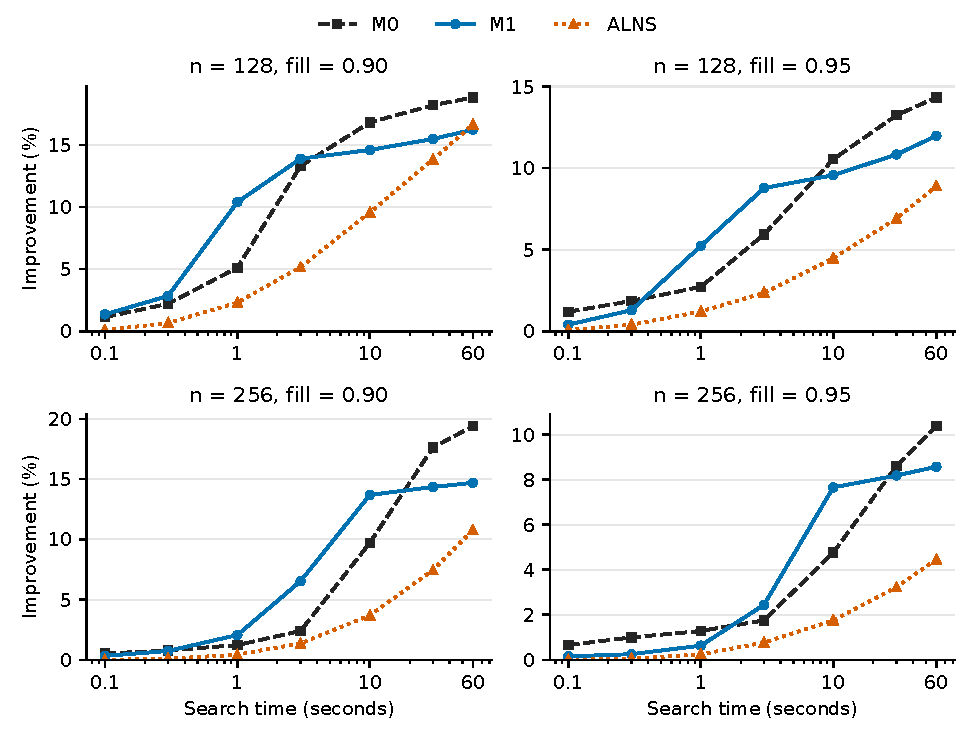
\includegraphics[width=\linewidth]{fig_extended_anytime.pdf}
\caption{Quality through 60 seconds for 128 and 256 facilities. Points are
mean initial-objective improvements after averaging three seeds within
instance and giving the two geometry families equal weight. Each shorter
cutoff is a prefix of the same 60-second run; connecting lines guide the eye.
Time excludes the common initializer. Table~\ref{tab:extendedcontrasts}
gives pointwise intervals for the primary contrasts.}
\label{fig:extendedanytime}
\end{figure}

Figure~\ref{fig:extendedanytime} makes the tradeoff visible at the larger
sizes. Partial repair gives a useful early improvement at $n=256$, while
full regeneration continues to improve and overtakes it by 60 seconds.
Time-to-target summaries provide a related check. At $n=256$, fill 0.95,
M1 reaches a 5\% improvement in 94.2\% of runs with a restricted mean of
9.76 seconds, compared with 90.0\% and 20.73 seconds for M0. For the
more demanding target,
the fractions reaching a 10\% improvement within 60 seconds are 56.67\%
for M0, 20.00\% for M1, and zero for ALNS, pooling the two geometries.
Their restricted mean search times are 39.15, 51.74, and 60.00 seconds.
Thus M1's early quality advantage does not imply faster attainment of a
larger improvement target. Geometry-specific quality and coverage,
pooled target times, and complete quality curves are in the Online Supplement, S1.

\subsection{What partial repair contributes}
\label{sec:sharedresult}
The separate one-second mechanism study provides controls for the repair
operation. On its 196 initialized dense instances, M1 exceeds B1 by
5.93 percentage points (95\% paired interval 4.99 to 6.88). Its gains over
reuse without repair (R0), spatial repair (B2), and small spatial repair
(B2S) are 6.39, 7.02, and 6.33 points, respectively. M1 improves the
initial objective by 7.98\% to 9.65\% across the four geometry and size
cells, compared with 1.72\% to 4.44\% for B1. Detailed budget tables
are in the Online Supplement, S2.

Successful nonempty repairs account for 6,215 incumbent updates and 92\%
of M1's logged objective gain, compared with 1,380 updates from unchanged
reuse. Mean proposed displaced-set size ranges from 1.95 to 2.72, and
2.19\% to 3.91\% of attempted nonempty repairs of size at most four succeed.
These are descriptive mechanism counts, not independent inferential samples.
Together with the R0 contrast, they show that the repair branch carries
most of the improvement.

The pooled M1 minus M0 difference at one second is 0.25 points
($-0.42$ to 0.92). In the separate fill 0.90 boundary check, M0 leads
by 1.87 points (1.17 to 2.60) on 79 initialized instances. These results
complement, rather than pool with, the 60-second comparison.

\subsection{Verification and timing}
All 17,228 stored layouts in the 60-second study pass the independent audit,
with zero objective recomputation error. The audit also checks instance
identity, shared initialization, trace monotonicity, and cutoff eligibility.
No method records a final verification failure. Mean process-CPU to wall-time
ratios are 0.979 to 0.981, and their medians are 0.997 for all three methods.
The largest function-return overrun is 66.4 ms; completed candidates after the
deadline are excluded. The one-second studies are audited separately, with
8,820 dense and 5,214 boundary budget layouts verified. Detailed timing
distributions are reported in S1 and S2.


\subsection{Small-instance objective calibration}
\label{sec:results_bench}
To complement the paired rankings with bounds on objective quality, we freeze
a dedicated small plate family from the same
generator ($n=8$, fills $0.40$ to $0.75$, $20$ instances each, mean facility
area $6$ to $10$ so plates stay at $66$ to $195$ cells). The CP-SAT model
\citep{GoogleCPSAT} has
integer lower-left coordinates $X_i\in[0,W-w_i]$ and
$Y_i\in[0,H-h_i]$, interval variables of fixed size, and a native
\textsc{NoOverlap2D} constraint. For every nonzero pair, an allowed-assignment
table has columns $(u,v,q)$, where $u=X_j-X_i$, $v=Y_j-Y_i$, and
$q=\operatorname{round}(10^4 w_{\mathrm{adj}}c_{ij})$. Boundary coefficients are rounded at the
same scale and attached to reified wall-contact variables. The no-overlap bonus
is constant on $\cF$ and is added without rounding.

Let $a_\ell(g)$ denote an unrounded active pair or wall term, let $M$ be the
number of such terms and let $s=10^4$.
For every feasible layout,
\begin{equation}
 \widehat J(g)=\beta_{\max}+\frac{1}{s}
 \sum_{\ell=1}^{M}\operatorname{round}(s a_\ell(g)),
 \qquad |J(g)-\widehat J(g)|\le\delta:=\frac{M}{2s}.
\label{eq:quantbound}
\end{equation}
Thus a CP-SAT upper bound $\widehat U$ transfers to the real objective as
$U=\widehat U+\delta$, and an optimizer of $\widehat J$ is within $2\delta$ of
the real optimum. CP-SAT proves 45 of 60 \emph{quantized} models optimal within
600 seconds and returns bounds for the other 15. The audit independently checks
all returned layouts and reevaluates their real objective. The largest
$\delta$ is $0.00215$ and the largest observed $|J-\widehat J|$ is $0.000322$.
The real-valued guarantee is the transferred upper bound with its explicit
rounding allowance.

\begin{table}[t]
\centering
\caption{Small-instance calibration at $n=8$. The first three numeric columns
are real-objective shortfalls from the returned CP-SAT solution on the 45
quantized models proved optimal. The last column averages the relative gap
bounds obtained from the transferred real upper bound $U$ on the full set of
60 instances (59 feasible returns for regret 4); it is not a worst-case bound. Objectives and bounds are positive here, so
$(U-J)/U$ upper-bounds the relative gap to the unknown real optimum. Regret 4 is
infeasible on one instance and is excluded rather than imputed.}
\label{tab:gaps}
\small
\setlength{\tabcolsep}{4pt}
\begin{tabular}{@{}lrrrr@{}}
\toprule
method & mean & median & max & mean gap bound \\
\midrule
beam width 32          & \textbf{0.40\%} & \textbf{0.19\%} & 2.66\% & $\le$0.85\% \\
SA 45\,000, lattice    & 1.48\% & 0.85\% & 9.79\% & $\le$1.74\% \\
regret 4 insertion     & 1.94\% & 1.41\% & 6.05\% & $\le$2.35\% \\
tabu 45\,000, greedy start & 2.62\% & 1.96\% & 7.31\% & $\le$2.88\% \\
largest first greedy   & 2.77\% & 2.13\% & 7.31\% & $\le$3.00\% \\
\bottomrule
\end{tabular}
\end{table}

The ranking replicates the paired comparison on this small family. The bounds
calibrate objective quality at $n=8$ for the same objective. Optimality gaps for the larger layout instances and bounds for the separate
QAPLIB objective require their own studies.


\subsection{Secondary boundary studies}
\label{sec:results_density}
\label{sec:results_scale}
\label{sec:results_qap}
\label{sec:results_mcnc}
Secondary studies examine completion reliability and representation limits.
Unfiltered one-step construction loses completion reliability as fill approaches
0.95, showing the limits of local legality checks. Constructor feasibility tests
up to 256 facilities complement M1's quality evaluation in
Section~\ref{sec:extendedresults}. Under the QAPLIB objective, swap improvement
performs well when geometric feasibility constraints are absent. Tests on
integer-converted MCNC/GSRC floorplans assess direct lattice construction;
the conversion changes rectangle geometry and dead space, so the results
cannot be compared directly with published full-resolution floorplans.
Selected tables are in the Online Supplement and complete results are in the
archive. These studies provide context for the primary matched-time comparison.

%%%%%%%%%%%%%%%%%%%%%%%%%%%%%%%%%%%%%%%%%%%%%%%%%%%%%%%%%%%%%%%%%%%%%%%%%%%%%%
\section{Discussion}
\label{sec:discussion}

The main comparison identifies a practical role for partial repair: obtaining
an improved dense layout within a limited search budget. At fill 0.95, M1
outperforms the selected adaptive repair control at 10 and 60 seconds across
all four sizes. The one-second reuse control provides complementary evidence
that nonempty repairs, rather than simply retaining a feasible layout, account
for most of the improvement.

Full regeneration remains a competitive alternative. With 256 facilities,
partial repair gives higher quality at 10 seconds at both fills, while full
regeneration leads at 60 seconds. At 128 facilities, full regeneration also
leads at 60 seconds. Partial repair reduces the number of facilities passed
to the completion heuristic, but it fixes every unaffected rectangle and
rejects proposals that displace more than four facilities. The observed
crossover is consistent with this tradeoff between cheaper repair and a
smaller neighborhood. It does not establish that repair cost alone causes the
difference, since ranking, verification, and the sequence of accepted
placements also affect search.

These results matter when a planner compares several feasible alternatives
before choosing which designs deserve more computation. Partial repair can
provide an early improved candidate, while further search may favor full
regeneration. This interpretation concerns computational performance on the
tested instances; the experiments do not measure industrial decision times.
A time-dependent combination of repair and full regeneration is a natural
next question, but the present comparison does not evaluate such a hybrid.

The compatible completion and the best complete layout serve distinct roles.
The former supports the next commitment, while the latter protects output
quality. All compared methods retain a verified incumbent and therefore share
feasible-return coverage and non-worsening output after initialization. Their
quality differences measure the search operations performed with the remaining
time, not a difference in whether a feasible result is returned.

The small CP-SAT and QAPLIB studies provide complementary calibration. CP-SAT
bounds the same objective at $n=8$ with an explicit integer-to-real allowance.
QAPLIB shows that swap search is strong when geometric feasibility is absent.
Neither supplies an optimality bound for the dense 32- to 256-facility cells.

%%%%%%%%%%%%%%%%%%%%%%%%%%%%%%%%%%%%%%%%%%%%%%%%%%%%%%%%%%%%%%%%%%%%%%%%%%%%%%
\section{Limitations}
\label{sec:limitations}

\begin{enumerate}
\item \textbf{The tested regime is bounded.} The main study covers 32 to
256 facilities, two generated geometry families, and budgets through 60 seconds.
Each geometry and size cell has 20 attempts at fill 0.95 and 10 at fill 0.90,
with three seeds. The smaller fill 0.90 sample gives less precise estimates.
The pointwise intervals do not provide a simultaneous confidence statement
across all sizes, fills, controls, and cutoffs.

\item \textbf{Initialization remains incomplete.} The main study initializes
236 of 240 instances, including 18 of 20 in each $n=32$, fill 0.95 cell.
The one-second dense study initializes 196 of 200. Quality comparisons are
conditional on these common initialized sets; feasible instances can still
defeat the initializer.

\item \textbf{Repair neighborhood coverage.} The adaptive control combines
six operator pairs and uses a configuration chosen from four candidates on
16 validation instances. This is a defined layout-specific ALNS baseline,
not an exhaustive evaluation of adaptive search. Other operators, CP-SAT
repair, or more tuning may improve it. M1's cap of four and exact marginal
candidate order are also empirical choices.

\item \textbf{The representation and objective limit external validity.}
Core experiments use fixed-orientation axis-aligned rectangles on a lattice,
without corridors or doors. Rotation is enabled only in the MCNC/GSRC transfer
study. Integer conversion changes those benchmark geometries and prevents
direct comparison with full-resolution topological fixed-outline methods.
The 60-second study also increases plate capacity with facility count, so
size-dependent results concern this joint scaling of $n$ and the plate.

\item \textbf{Optimality evidence is local.} CP-SAT closes 45 of 60 scaled
integer models at $n=8$. The real-objective allowance is small but nonzero,
and neither these bounds nor QAPLIB optima transfer to larger sizes or
another objective.

\item \textbf{Timing depends on the execution setting.} The main study uses
eight pinned single-threaded workers, not an otherwise idle single-worker
machine. The one-second study uses a separate software environment. These
timings are kept separate. Learned inference appears only in secondary
GPU diagnostics and is not a hardware-normalized speedup over CPU search.
\end{enumerate}

%%%%%%%%%%%%%%%%%%%%%%%%%%%%%%%%%%%%%%%%%%%%%%%%%%%%%%%%%%%%%%%%%%%%%%%%%%%%%%
\section{Conclusion}
\label{sec:conclusion}

This paper develops completion-aware search with partial witness repair for
dense fixed-shape facility layout. A proposed placement determines which
witness rectangles must move, while every compatible rectangle is reused.
An independent verifier checks complete candidates, and a separate best
layout protects the quality of the returned solution.

The main study evaluates M1, full completion regeneration, and a
validation-selected adaptive repair control on 240 attempted instances with
up to 256 facilities. At fill 0.95, M1 exceeds the adaptive control by
3.45 to 5.91 percentage points in initial-objective improvement at 10 seconds
and 1.68 to 4.12 points at 60 seconds. With 256 facilities at this fill,
M1 gives 7.66\% improvement at 10 seconds, compared with 4.76\% for full
regeneration. By 60 seconds, full regeneration gives 10.38\%, compared with
8.58\% for M1. The separate one-second study attributes most of M1's gain
to nonempty repair rather than unchanged reuse.

Partial witness repair is therefore useful for early improvement in dense
packing, while broader reconstruction can produce a better solution with more
time. The experiments make this choice explicit in terms of size, density,
and search budget.

%%%%%%%%%%%%%%%%%%%%%%%%%%%%%%%%%%%%%%%%%%%%%%%%%%%%%%%%%%%%%%%%%%%%%%%%%%%%%%
\ifdefined\CIEAuthorCopy
\section*{Acknowledgements}
Yeoneung Kim is supported by the National Research Foundation of Korea (NRF)
grants funded by the Korea government (MSIT) (RS-2023-00219980,
RS-2026-25490291) and Yonsei University.

The funders had no role in study design; data collection, analysis and
interpretation; manuscript preparation; or the decision to submit the article
for publication.

\AuthorContributions
\fi

\section*{Data and code availability}
\ifdefined\CIEAuthorCopy
The code and data supporting this study are publicly available at
\url{https://github.com/yeoneung/layout_optimization}.
The repository includes benchmark generators and instances, trained policies,
experimental results, and analysis and verification scripts.

\else
The benchmark generators, experimental results, and analysis and verification
scripts are documented in the accompanying research materials. Identifying
repository details are provided separately to the editorial office.
\fi

\section*{Supplementary material}
The Online Supplement reports the primary 60-second comparison, including
adaptive repair configuration, coverage, geometry-specific quality, target
times, and timing checks (S1), followed by the one-second repair-mechanism
study (S2). Secondary comparisons cover transfer, quality and diversity,
amortized cost, reward and action configurations, completion checks, and
constructor feasibility (S3 to S10). Feasibility, initialization, and selector
comparisons are in S11; secondary methods and dataset coverage are in S12;
policy architecture and training costs are in S13.

\section*{Declaration of competing interests}
The authors declare no conflicts of interest.

\appendix
%%%%%%%%%%%%%%%%%%%%%%%%%%%%%%%%%%%%%%%%%%%%%%%%%%%%%%%%%%%%%%%%%%%%%%%%%%%%%%
\section{Objective definition}
\label{app:objective}
\paragraph{Adjusted distance}
Write $c_i$ for facility $i$'s center and $t=|\Delta y|/|\Delta x|$ for the
slope of the segment joining the two centers. The directional radius $r_i$ is
the distance from $c_i$ to the boundary of $i$'s rectangle along that segment:
the ray exits through a vertical edge when $t\le h_i/w_i$, at offsets
$(w_i/2,\,t\,w_i/2)$ from the center, and through a horizontal edge otherwise,
at offsets $(h_i/2t,\,h_i/2)$; $r_i$ is the Euclidean norm of the offsets. The
adjusted distance is $d_{ij}=\lVert c_j-c_i\rVert_2-r_i-r_j$, which is zero
when the rectangles touch along the segment. Its normalizer $\bar d_{ij}$ is
the same quantity evaluated with $c_i$ at its lower left extreme
$(w_i/2,h_i/2)$ and $c_j$ at its upper right extreme $(W-w_j/2,H-h_j/2)$,
floored at $10^{-12}$.

\paragraph{Pair and boundary terms}
With $\nu_{ij}=\min(d_{ij}/\bar d_{ij},1)^{\rho}$,
\[
c_{ij}=\begin{cases}A_{ij}\,\nu_{ij} & A_{ij}\ge 0\\ -A_{ij}\,(1-\nu_{ij}) & A_{ij}<0,\end{cases}
\]
zeroed if $i$ and $j$ overlap. The boundary term is
\begin{align*}
b_i \;=\;& w_{\mathrm e}\,h_i\,s_i\,\mathbf 1[\text{$i$ flush left or right}]\\
 &+ w_{\mathrm e}\,w_i\,p_i\,\mathbf 1[\text{flush bottom}]
  + w_{\mathrm e}\,w_i\,q_i\,\mathbf 1[\text{flush top}],
\end{align*}
where $(s_i,p_i,q_i)\in\{0,1\}^3$ is the wall preference archetype of $i$'s
type; $b_i$ is zeroed whenever $i$ overlaps anything.

\paragraph{Constants and the terms off $\cF$}
The constants are $w_{\mathrm{adj}}=w_{\mathrm e}=2$ and $\rho=1$. With
$A(g)$ the total pairwise overlap area and $P=w_{\mathrm{ov}}A(g)$, the full
evaluator is the pair sum plus the boundary sum plus $P+B(P)$. Here
$w_{\mathrm{ov}}=-8$ and
\[
B(P)=\begin{cases}
\beta_{\max}=400, & P=0,\\
\beta_{\mathrm{mid}}(1-P/\tau)^2, & \tau\le P<0,\\
0, & P<\tau,
\end{cases}
\]
where $\beta_{\mathrm{mid}}=200$ and $\tau=-200$. Therefore $P=0$ and
$B(P)=\beta_{\max}$ on $\cF$, exactly as in Eq.~\eqref{eq:objective}; off
$\cF$, the overlap penalty and graded bonus apply.

\paragraph{Generated suite distributions}
Each instance draws its mean facility area from $U(9,30)$, capped at $0.95$ of
the budget for each facility, $G^2\cdot\mathrm{fill}/n$; a plate aspect ratio from
$U(1,1.8)$; plate sides meeting the implied area, each at most $G$;
$G=44$ in the one-second study and $G=44,44,72,100$ for
$n=32,64,128,256$, respectively, in the 60-second study; a
guillotine partition with minimum side $2$, shrunk to the target fill; a type
count $T$ uniform on $\{6,\dots,\min(12,n)\}$; a symmetric integer affinity
table on types, entries uniform on $\{-8,\dots,8\}$ and zeroed with
probability $0.25$; and a wall preference archetype per type. Three objective
constants are drawn again once per suite cell, spanning the range the two
reference scenarios occupy: $w_{\mathrm{ov}}\sim U(-12,-6)$,
$\beta_{\max}\sim U(320,520)$ and $\tau\sim U(-280,-160)$; all other constants
are fixed at the values above.

\section*{Declaration of generative AI and AI-assisted technologies in the
manuscript preparation process}
During the preparation of this work, the authors used OpenAI Codex and Anthropic
Claude for language editing, implementation assistance, and checking of
numerical consistency. After using these tools, the authors reviewed and edited
the content as needed and take full responsibility for the content of the
publication.

\printbibliography

\end{document}
